\documentclass[12pt]{article}  % 字号:12号

%\usepackage{fancyhdr}
%\pagestyle{fancy}
%\lhead{}

\usepackage{subfigure}
\usepackage{graphicx}
\usepackage[2115291]{easymcm}

\usepackage{pxfonts}

\usepackage{minted}

\begin{document}
\begin{center}
\begin{LARGE}
\textbf{SUSTech Store - Project Proposal}
\end{LARGE}

\vspace{20pt}
\begin{large}
% \qquad \textbf{Name:} Liu Jidong \qquad  Tan Yajing\\
% \vspace{10pt}
% \textbf{Student ID:} 11910831 \qquad 11911336
\begin{center}
	\begin{tabular}{rl}
	% after \\: \hline or \cline{col1-col2} \cline{col3-col4} ...
	
	
	Liu Jidong & 11910831 \\
	Tan Yajing & 11911336 \\
	Hou Yilin & 11912636 \\
	Wei Fenglin & 11811323 \\
	Xu Zhuolin & 11912933
	\end{tabular}
  \end{center}


\end{large}

\vspace{20pt}

\begin{Large}
\textbf{Executive Abstract}
\end{Large}
\end{center}

\begin{large}
	The project is to provide a convenient web service 
for student in SUSTech to buy and sell secondhand goods. 
Three of us will focus on designing the front-end page 
and the other two will focus on back-end part. 

We've already drawn the draft of pages, specified the page 
jumping logic, finished API document and drawn the 
database ER diagram. The appearance and function of 
different pages are divided into three parts and each 
member of front end group will finish one of them. 

At the meantime, the back end group will implement 
the function specified in the API document. We will 
try to connect front end with back end for a few pages 
before 11.1 and more detail about our work plan is in 
the Time line part.
\end{large}

\vspace{30pt}

\tableofcontents

%正文
\section{Group Information}

Front-End: Liu Jidong, Tan Yajing, Hou Yilin

Back-End: Wei Fenglin, Xu Zhuolin

\section{Description}

\subsection{Motivation}

Many secondary market QQ groups exist in Southern University 
of Science and Technology. However, Students' posting and 
requesting goods are always quickly flooded with messages in 
QQ group, and it is not convenient for students to search for 
the goods. 

Therefore, we plan to develop the SUSTech Store Web Service. 
Buyers can search for the products posted by sellers directly 
through the search box . It will be more convenient to buy and 
sell second-hand goods.


\subsection{Feature Description}

\subsubsection*{Use Case Diagram:}

\begin{figure}[!htbp]
	\centering
	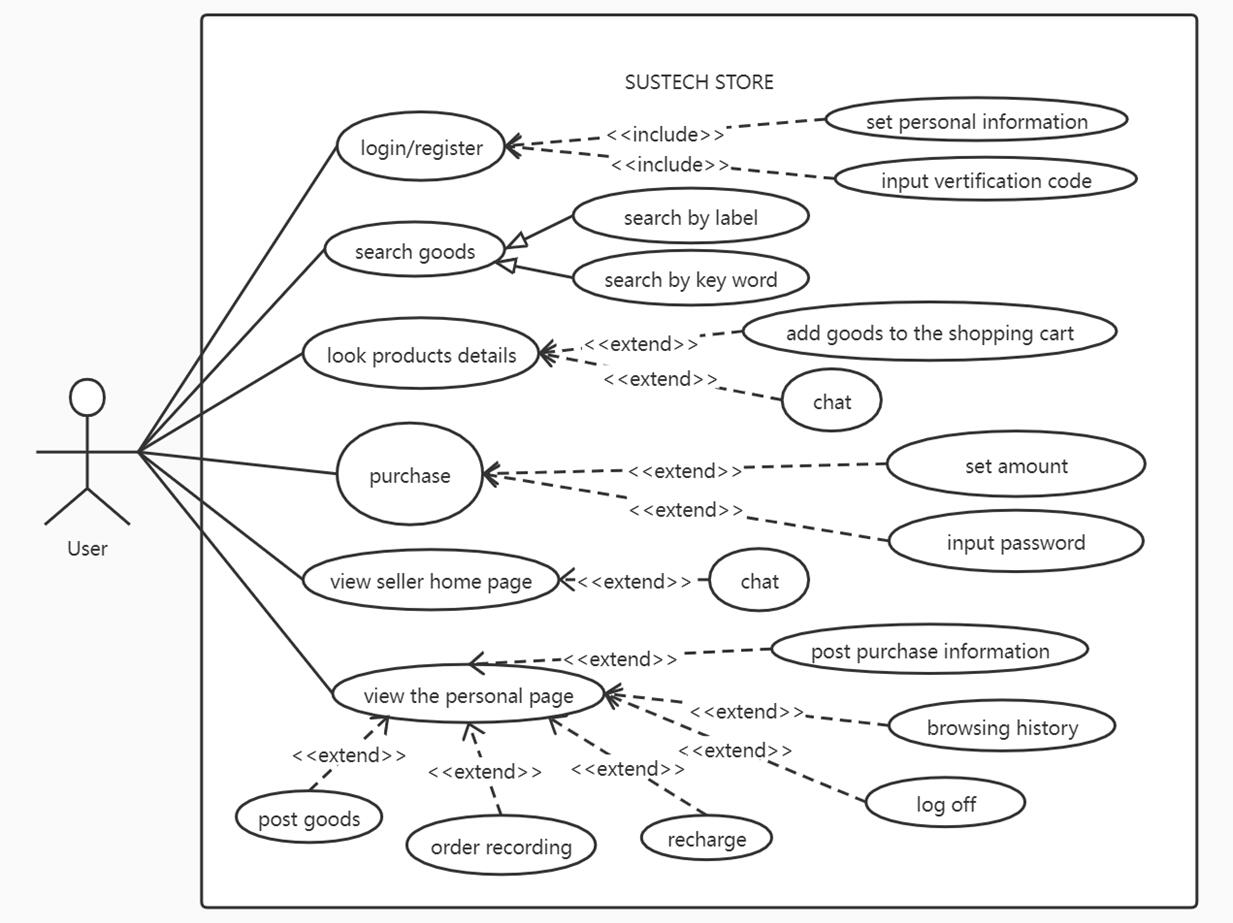
\includegraphics[width=0.8\textwidth]{images/useCaseDiagram.jpg}
	\caption{Use Case Diagram}
\end{figure}

As the use case diagram shows, the process of using our SUSTech 
Store web service is as follows:

First, the user should register for an account first. The web 
will send him a verify code via Email. Then he can login and 
start to use the SUSTech Store Web Service.

If he/she(following will be represented by B) acts as a buyer, 
B can search goods he wants to buy by label or by keyword 
in search box. Then after he click the product, he can look 
the product's details. Then he can chat with the seller for 
further information or add the products directly to the 
shopping cart. 

When purchasing, he should set the amount 
and enter password for security. Then an email will be sent 
to B's register email also for security. He can view his 
personal page for previous order, recharging, browsing 
transaction history, and post purchase information.

If B acts as a seller, he can post goods via his personal 
page and do all the things buyer's can do. Because students 
usually acts as both seller and buyer.




\subsection{Requirements}
\subsubsection*{Login/Register}
- send a verification code to the register email

- verify the validation of register information

- encrypt the password in the database to avoid user 
information leakage

\subsubsection*{Search and Buy goods}
+ select data from database by the condition given 
by buyer

+ when buying goods, check user's balance and the 
remaining number of goods to verify the validation 
of the transaction

+ transaction needs password and send email to inform 
the user to avoid other people using account to buy 
things

+ transaction history is stored and can be viewed 
in personal page

+ if the goods buyers want to purchase are not in 
the platform, he can post purchase information

+ recharge virtual currency

+ can chat with sellers, the platform will store 
their chatting records
\subsubsection*{Seller part}
- can post goods, the platform will add it to 
the database

- can chat with buyers, the platform will store 
their chatting records

- credit is set to evaluate sellers' quality

\subsection{Design Document}
\subsubsection*{Class Diagram:}
\begin{figure}[H]
	\centering
	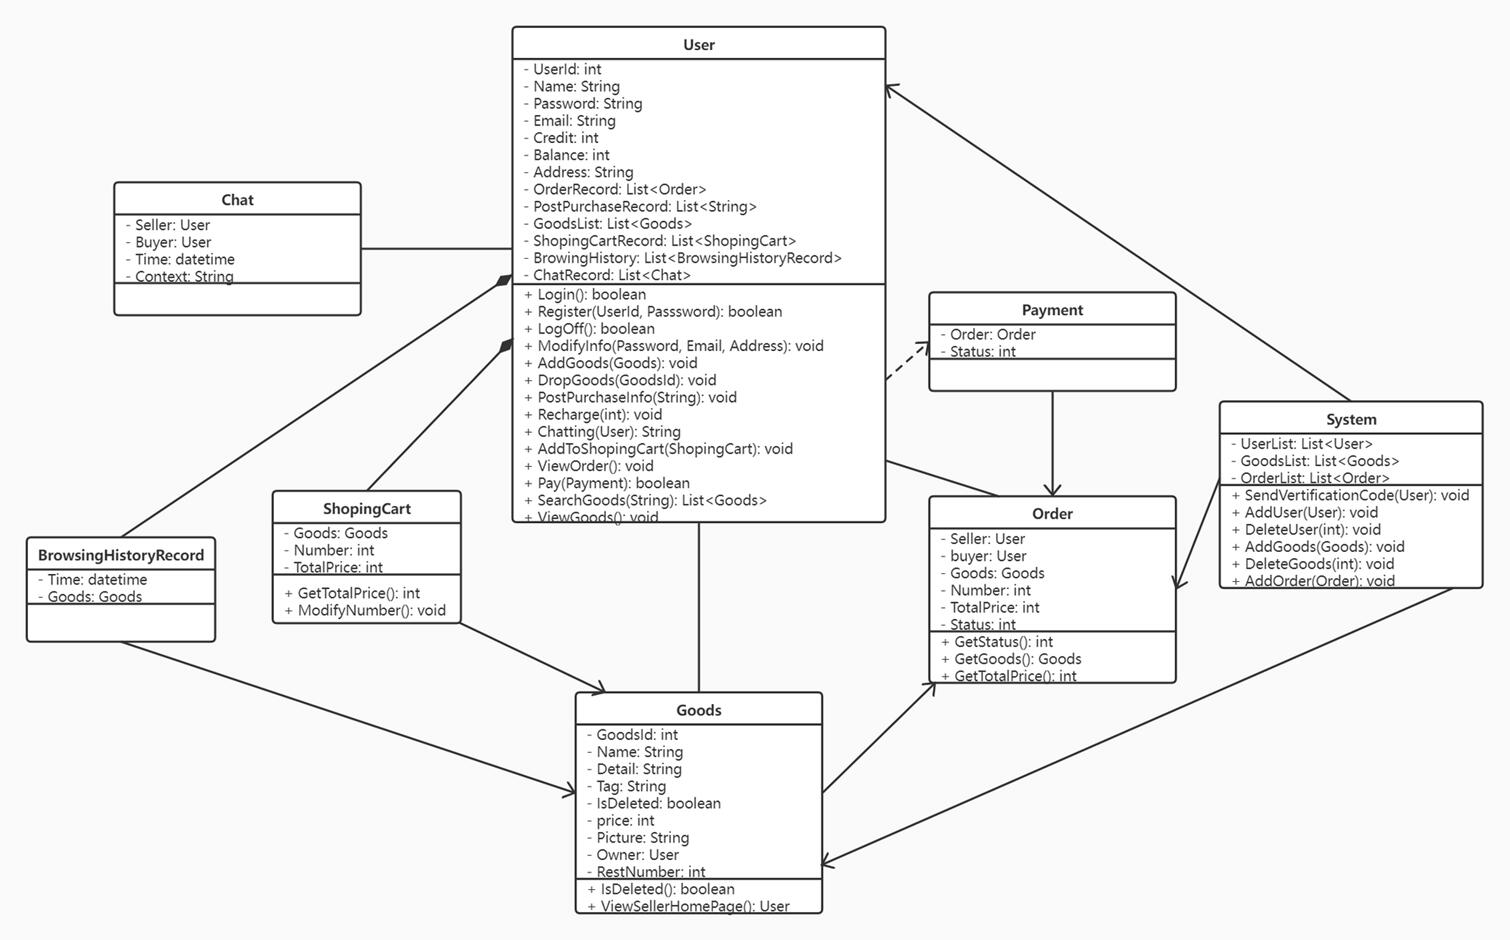
\includegraphics[width=0.8\textwidth]{images/classDiagram.jpg}
	\caption{Class Diagram}
\end{figure}

\subsubsection*{ER Diagram: }
\begin{figure}[H]
	\centering
	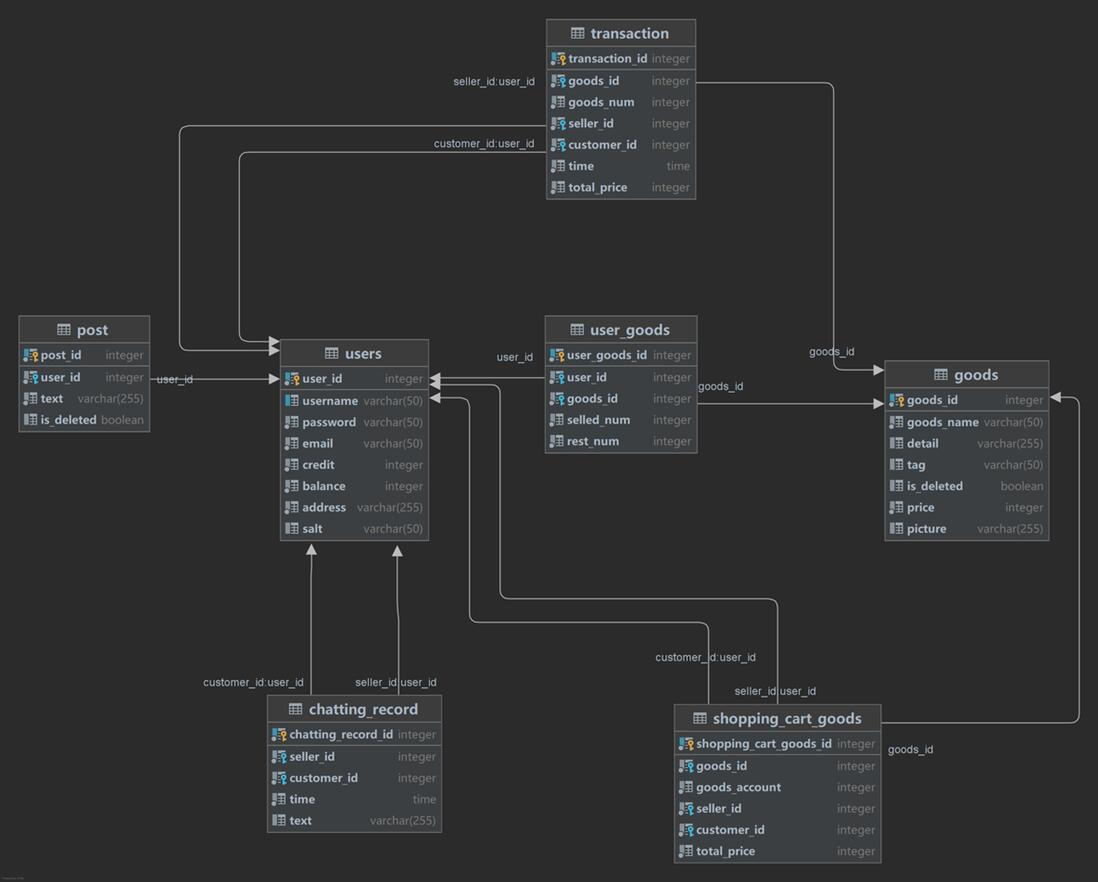
\includegraphics[width=0.8\textwidth]{images/ERDiagram.jpg}
	\caption{ER Diagram}
\end{figure}



\subsection{Feasibility}

We divided the feature into basis features and advanced 
features, and we plan to first implement basic features, 
if time permitted, we will try to implement advanced 
features.

Basic features:

Login/Register, Main Page, Personal Home Page, Search Box, 
Goods Details, Mail Reminder, Chatting, Release and Post 
Goods, Transaction, Pay by Virtual Currency, Credit...

Advanced features:

Seller Home Page, Shopping Cart, Browsing History, 
Recommending Goods

\section{Techniques}
\begin{large}
	\textbf{Vue: }
\end{large}
It is a set of progressive JavaScript frameworks for 
building user interfaces. 


\begin{large}
	\textbf{Spring Boot: }
\end{large}
Spring is a lightweight container that manages the life 
cycle of beans. It provides powerful IOC, AOP and Web 
MVC functions. SpringBoot simplifies the initial setup 
and development of new Spring applications. 

\section{API}
\subsubsection*{Authentication APIs}
Login: $POST\sim/api/login$

Logout: $POST\sim/api/logout$

Register: $POST\sim/api/register$

\subsubsection*{Homepage APIs}

Query by tag: $GET\sim/api/view\_by\_tag$

Query by name: $GET\sim/api/view\_by\_name$

Get a specific goods: $GET\sim/api/view\_goods/{goods\_id}$

\subsubsection*{Searching Results APIs}

Query by conditions: $GET\sim/api/searching$

Get a specific goods: $GET\sim/api/view\_goods/{goods\_id}$

\subsubsection*{Goods description APIs}

Chat with seller: $GET\sim/api/start\_chatting/{id}$

Add to shopping cart: $POST\sim/api/add\_to\_cart$

\subsubsection*{Chatting APIs}

View chatting record: $GET\sim/api/chat\_record/chat/{id}/seller/{id}$

Post chatting content: $POST\sim/api/chat/{id}/seller/{id}$

\vspace{-10pt}

\subsubsection*{Confirm order APIs}

Buy the goods: $POST\sim/api/buy/{goods\_id}$

Check password again: $POST\sim/api/pay\_password/{id}$

Recharge: $POST\sim/api/recharge{id}$

\vspace{-10pt}

\subsubsection*{Personal Homepage APIs}

Query user's basic info: $GET\sim/api/mainpage/{id}$

Query posted record: $GET\sim/api/posted\_record/{id}$

Query sales record: $GET\sim/api/sales\_record/{id}$

Query purchase record: $GET\sim/api/purchase\_record/{id}$

Recharge: $POST\sim/api/recharge{id}$

Modify info: $POST\sim/api/modify\_info{id}$

\vspace{-10pt}

\subsubsection*{Release New Message APIs}
Post new goods/post : $POST\sim/api/post\_new/{id}$

\vspace{-10pt}

\subsubsection*{View history buy/post record APIs}
Query record: $GET\sim/api/purchase\_record/{id}$

% \vspace{-15pt}

\section{Timeline}

Before 11.1: 
First attempt to connect front-end with 
back-end on a few pages. Get the user basic info, goods 
info from database and show them in corresponding pages. 
Post goods and store them into database. Implement 
logout function.

Before 11.7: 
Finish the design idea of all front-end pages, including 
where the buttons, text, pictures and the tables should 
be settled. Implement the recharge and modify 
personal info function. Implement displaying selected 
goods after searching. 

Before 11.21:
Complete the appearance of all front-end 
page components. Implement checking various 
records(e.g. transaction record).

Before 12.5:
Finish online chatting function and the credit system. 
Implement all API.

Before 12.12:
Connect the whole front-end with back-end, finish the 
basic functions of the website.

Before 12.19:
Adding elements related to SUSTech, improve the 
security and try to support purchasing agent service.




\end{document}




